\documentclass[compacto,10pt]{pubciencias-notas}

% -- Paquetes adicionales
\usepackage{comandosEPN}
\usepackage{tikz}
\usetikzlibrary{babel}

% -- Datos del libro
\autor{Departamento de Formación Básica}
\materia{Álgebra Lineal}
\nota{Semana 04 Clase 02}
\fecha{Semestre 2026-B}

\logouno[1.1cm]{Logo_EPN.eps}
\logodos[1.7cm]{Logo_DFB.eps}

\definecolor{colordef}{cmyk}{0.81,0.62,0.00,0.22}

\begin{document}

\encabezado

\vspace*{-8mm}

\setcounter{section}{2}
\section{Determinantes}
\subsection{Motivación: Deformaciones del espacio. El determinante como factor de escalamiento}

Al multiplicar una matriz cuadrada por un vector en $\mathbb{R}^2$, esta actúa asignando a cada punto una nueva posición en el plano, lo que produce deformaciones geométricas sobre las figuras: puede estirarlas, rotarlas o incluso comprimirlas. Para comprender esta acción sobre el espacio, tomemos como referencia el cuadrado unitario delimitado por los vértices $(0,0)^{\top}$, $(1,0)^{\top}$, $(0,1)^{\top}$ y $(1,1)^{\top}$, y analicemos cómo distintas matrices modifican su área.

Por ejemplo, consideremos la matriz
\[
    A = \begin{pmatrix} 3 & 0 \\ 0 & 1 \end{pmatrix}.
\]
Al multiplicar $A$ por cada uno de los cuatro vértices del cuadrado unitario, obtenemos $(0,0)^{\top}$, $(3,0)^{\top}$, $(0,1)^{\top}$ y
$(3,1)^{\top}$, respectivamente. Por tanto, el cuadrado unitario se convierte en un rectángulo de lados 3 y 1, cuya área es 3. En otras palabras, la transformación dada por $A$ multiplica el área inicial por 3; este factor se identifica como $|\det(A)|$, es decir, $|\det(A)|=3$.
\begin{center}
\begin{minipage}[t]{0.42\textwidth}
    \centering
    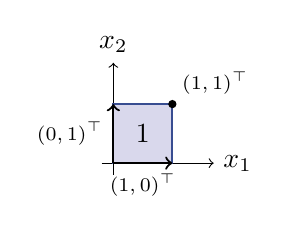
\begin{tikzpicture}[scale=0.75]
        \draw[->] (-0.2,0)--(1.7,0) node[right] {$x_1$};
        \draw[->] (0,-0.2)--(0,1.7) node[above] {$x_2$};
        \filldraw[fill=colordef!15,draw=colordef,thick]
            (0,0)--(1,0)--(1,1)--(0,1)--cycle;
        \draw[->,thick] (0,0)--(1,0)
            node[midway,below] {\scriptsize$(1,0)^{\top}$};
        \draw[->,thick] (0,0)--(0,1)
            node[midway,left] {\scriptsize$(0,1)^{\top}$};
        \fill (1,1) circle (2pt);
        \node[above right] at (1,1) {\scriptsize$(1,1)^{\top}$};
        \node at (0.5,0.5) {$1$};
    \end{tikzpicture}

    Cuadrado unidad
\end{minipage}
\hfill
\begin{minipage}[t]{0.42\textwidth}
    \centering
    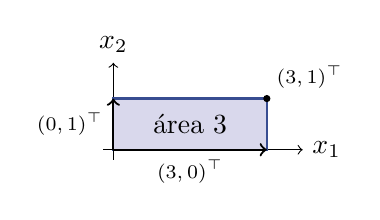
\begin{tikzpicture}[scale=0.65]
        \draw[->] (-0.2,0)--(3.7,0) node[right] {$x_1$};
        \draw[->] (0,-0.2)--(0,1.7) node[above] {$x_2$};
        \filldraw[fill=colordef!15,draw=colordef,thick]
            (0,0)--(3,0)--(3,1)--(0,1)--cycle;
        \draw[->,thick] (0,0)--(3,0)
            node[midway,below] {\scriptsize$(3,0)^{\top}$};
        \draw[->,thick] (0,0)--(0,1)
            node[midway,left] {\scriptsize$(0,1)^{\top}$};
        \fill (3,1) circle (2pt);
        \node[above right] at (3,1) {\scriptsize$(3,1)^{\top}$};
        \node at (1.5,0.5) {área $3$};
    \end{tikzpicture}

    $A$ estira el área
\end{minipage}
\end{center}
En cambio, si realizamos el mismo procedimiento con la matriz 
\[
    B = \begin{pmatrix} 1 & 2 \\ 2 & 4 \end{pmatrix},
\]
los vectores resultantes al multiplicar $B$ por los vértices del cuadrado unitario son $(0,0)^{\top}$, $(1,2)^{\top}$, $(2,4)^{\top}$ y $(3,6)^{\top}$ (verifíquelo). Observe que todos estos puntos son colineales, por lo que la región bidimensional se reduce a un simple segmento de recta.

\begin{center}
\begin{minipage}[t]{0.52\textwidth}
    \centering
    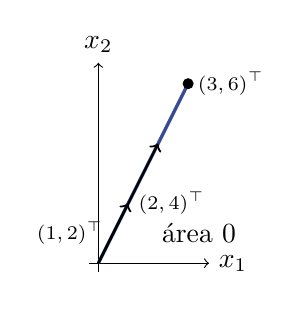
\begin{tikzpicture}[x=0.38cm,y=0.38cm]
        \draw[->] (-0.3,0)--(3.7,0) node[right] {$x_1$};
        \draw[->] (0,-0.3)--(0,6.7) node[above] {$x_2$};
        \draw[colordef,very thick] (0,0)--(3,6);
        \draw[->,thick] (0,0)--(1,2)
            node[midway,left] {\scriptsize$(1,2)^{\top}$};
        \draw[->,thick] (0,0)--(2,4)
            node[midway,right] {\scriptsize$(2,4)^{\top}$};
        \fill (3,6) circle (2pt);
        \node[right] at (3,6) {\scriptsize$(3,6)^{\top}$};
        \node[right] at (1.8,1) {área $0$};
    \end{tikzpicture}

    $B$ colapsa el área
\end{minipage}
\end{center}
En este caso, el segmento generado tiene área 0. Así,
\[
    |\det(B)|=0.
\]
La transformación dada por $B$ produce una pérdida de información al comprimir todo el plano sobre una recta, lo cual impide recuperar los vectores originales y explica por qué esta matriz no tiene inversa.

Estos ejemplos ilustran la interpretación geométrica de lo que definiremos como \emph{determinante}. Para una matriz cuadrada $M$, el área de la figura transformada satisface
\[
    \text{área transformada}
    =|\det(M)|\,\text{área original}.
\]
El valor absoluto $|\det(M)|$ es el factor de cambio de área, mientras que el signo de $\det(M)$ indica si la orientación se conserva o se invierte. En dimensiones mayores, el determinante cumple el mismo papel.

En general,
\[
    \det(M)\ne0
    \quad\Longleftrightarrow\quad
    M\text{ es invertible}.
\]
Así, el determinante también permite decidir si un sistema cuadrado posee una solución única para cada lado derecho.

A continuación, definiremos formalmente el determinante y presentaremos algunas de sus propiedades más importantes.

\subsection{Definiciones fundamentales}

\setcounter{defi}{0}
\begin{defi}[Menor]\label{sem04cl02:def-menor}
    Sea $A\in\Mat[\R]{n}{n}$. La matriz que se obtiene al eliminar la fila
    $i$ y la columna $j$ de $A$ se llama \textbf{menor $(i,j)$} de $A$ y se
    denota por $A_{ij}$. Esta matriz tiene tamaño $(n-1)\times(n-1)$.
\end{defi}

\begin{ejem}
    Si
    \[
        A=\begin{pmatrix}-1&4&0\\2&1&-2\\0&3&5\end{pmatrix},
    \]
    entonces
    \[
        A_{12}=\begin{pmatrix}2&-2\\0&5\end{pmatrix},
        \qquad
        A_{23}=\begin{pmatrix}-1&4\\0&3\end{pmatrix},
        \qquad
        A_{31}=\begin{pmatrix}4&0\\1&-2\end{pmatrix}.
    \]
\end{ejem}

\begin{advertencia}
    En algunos textos, ``menor'' designa el número $\det(A_{ij})$. En estos
    apuntes, $A_{ij}$ denota la matriz obtenida al eliminar una fila y una
    columna.
\end{advertencia}

\begin{defi}[Determinante]\label{sem04cl02:def-determinante}
    Sea $A=(a_{ij})\in\Mat[\R]{n}{n}$. El \textbf{determinante} de $A$,
    denotado por $\det(A)$, se define recursivamente:
    \begin{itemize}
        \item Si $n=1$ y $A=(a_{11})$, entonces $\det(A)=a_{11}$.
        \item Si $n>1$, el \textbf{cofactor $(i,j)$} de $A$ es
              \[
                  C_{ij}=(-1)^{i+j}\det(A_{ij}).
              \]
              Al escoger cualquier fila $i$, el determinante se calcula como
              la suma expandida
              \[
                  \det(A)=a_{i1}C_{i1}+a_{i2}C_{i2}+\cdots+a_{in}C_{in}.
              \]
              También se puede escoger cualquier columna $j$ y calcular
              \[
                  \det(A)=a_{1j}C_{1j}+a_{2j}C_{2j}+\cdots+a_{nj}C_{nj}.
              \]
    \end{itemize}
    Cada una de estas expresiones se llama \textbf{expansión por cofactores}
    de la fila o columna elegida.
\end{defi}

\begin{obs}
    Notar que el signo de los cofactores cambia de acuerdo con la suma de los índices: $(-1)^{i+j}$. En general, se alternan entre positivo y negativo. Para una matriz de tamaño $3\times3$, los signos se organizan de la siguiente manera:
    \[
        \begin{pmatrix}
            +&-&+\\
            -&+&-\\
            +&-&+
        \end{pmatrix}.
    \]
\end{obs}
\begin{ejem}[Determinante de una matriz \(2\times2\)]
    Sea
    \[
        A=\begin{pmatrix}a&b\\c&d\end{pmatrix}.
    \]
    El menor $(1,1)$ es $A_{11}=(d)$ y el menor $(1,2)$ es $A_{12}=(c)$. Por
    tanto, los cofactores son
    \[
        C_{11}=(-1)^{1+1}\det(A_{11})=d,
        \qquad
        C_{12}=(-1)^{1+2}\det(A_{12})=-c.
    \]
Para una matriz de tamaño $2\times2$, expandir por la primera fila da
\begin{align*}
    \det\begin{pmatrix}a&b\\c&d\end{pmatrix}
    &=aC_{11}+bC_{12}\\
    &=a\det(d)-b\det(c)\\
    &=ad-bc.
\end{align*}
\end{ejem}
\begin{advertencia}
    \textbf{Fórmula del determinante para matrices \(2\times2\)}
    
    \[\det\begin{pmatrix}a&b\\c&d\end{pmatrix}=ad-bc\]
\end{advertencia}

\begin{ejem}[Elección de una fila conveniente]
    Para
    \[
        B=\begin{pmatrix}1&2&0\\0&3&0\\4&-1&2\end{pmatrix},
    \]
    conviene escoger la segunda fila porque contiene dos ceros. La expansión
    completa por esta fila es
    \begin{align*}
        \det(B)
        &=0C_{21}+3C_{22}+0C_{23}\\
        &=3(-1)^{2+2}\det(B_{22})\\
        &=3\det\begin{pmatrix}1&0\\4&2\end{pmatrix}\\
        &=3(1\cdot2-0\cdot4)=6.
    \end{align*}
    La elección de una fila o columna con varios ceros reduce el número de
    cofactores que debemos calcular.
\end{ejem}

\subsection{Propiedades básicas}

Las siguientes propiedades permiten calcular determinantes sin desarrollar
siempre todos los menores.

\begin{prop}[Efecto de las operaciones por fila]\label{sem04cl02:prop-filas}
    Sea $A$ una matriz cuadrada.
    \begin{enumerate}
        \item Intercambiar dos filas cambia el signo del determinante.
        \item Multiplicar una fila por $c$ multiplica el determinante por $c$.
        \item Sumar a una fila un múltiplo de otra no cambia el determinante.
    \end{enumerate}
\end{prop}

\begin{prop}[Propiedades del determinante]
    Si $A,B\in\Mat[\R]{n}{n}$, entonces:
    \begin{enumerate}
        \item $\det(I_n)=1$;
        \item $\det(A^{\top})=\det(A)$;
        \item $\det(AB)=\det(A)\det(B)$;
        \item si $A$ es triangular, $\det(A)$ es el producto de las entradas
              de su diagonal.
    \end{enumerate}
\end{prop}

\begin{ejem}[Determinante mediante eliminación]
    Sea
    \[
        C=\begin{pmatrix}1&2&1\\2&1&0\\1&0&1\end{pmatrix}.
    \]
    Las operaciones $-2F_1+F_2\to F_2$ y
    $-F_1+F_3\to F_3$ no cambian el determinante:
    \[
        C\sim\begin{pmatrix}1&2&1\\0&-3&-2\\0&-2&0\end{pmatrix}
        \sim\begin{pmatrix}1&2&1\\0&-3&-2\\0&0&\frac{4}{3}\end{pmatrix},
    \]
    donde $-\frac{2}{3}F_2+F_3\to F_3$. Como la matriz final es
    triangular,
    \[
        \det(C)=1(-3)\frac{4}{3}=-4.
    \]
\end{ejem}

\begin{teo}[Determinante e invertibilidad]\label{sem04cl02:teo-invertible}
    Sea $A\in\Mat[\R]{n}{n}$. La matriz $A$ es invertible si y solo si
    \[
        \det(A)\ne0.
    \]
    Si $A$ es invertible, entonces
    \[
        \det(A^{-1})=\frac{1}{\det(A)}.
    \]
\end{teo}

En efecto, $AA^{-1}=I_n$ implica
\[
    \det(A)\det(A^{-1})=\det(I_n)=1.
\]
Por tanto, una matriz con determinante cero no puede tener inversa. Este
criterio conecta directamente los determinantes con la clase anterior.

\section{Ejercicios}

\begin{ejer}
    Calcule el determinante de cada matriz usando el método indicado y decida
    si es invertible.
    \begin{enumerate}
        \item $\begin{pmatrix}3&-1\\2&4\end{pmatrix}$, mediante la fórmula de
              orden dos.
        \item $\begin{pmatrix}1&0&2\\0&3&0\\-1&0&4\end{pmatrix}$, mediante
              expansión por cofactores.
        \item $\begin{pmatrix}1&2&3\\2&4&7\\0&1&1\end{pmatrix}$, mediante
              operaciones por fila.
    \end{enumerate}
\end{ejer}

\begin{ejer}[Aplicación]
    Una transformación del plano está representada por
    $T=\begin{pmatrix}2&1\\1&2\end{pmatrix}$. Determine el factor por el que
    cambia las áreas, indique si invierte la orientación y decida si es
    posible recuperar un vector original a partir de su imagen.
\end{ejer}

\end{document}
